Per l'esecuzione del'esperienza è stato utilizzato il seguente apparato sperimentale:
\begin{itemize}
    \item Termometro di vetro
    \item Termometro digitale
    \item Cronometro digitale
    \item 2 Becher
    \item Acqua
    \item Fornellino
\end{itemize}

\begin{table}[H]
	\centering
	\begin{tabular}{|c|c|}
		\hline
		\textbf{Strumenti di misura} & \textbf{Risoluzione} \\
		\hline
		Cronometro digitale & $0.01\ s$ \\
		Termometro digitale & $0.1\ \,^\circ\mathrm{C}$ \\
		\hline
	\end{tabular}
	\caption{Risoluzione degli strumenti di misura utilizzati}
	\label{tab:}
\end{table}

\begin{figure}[H]
	\centering
	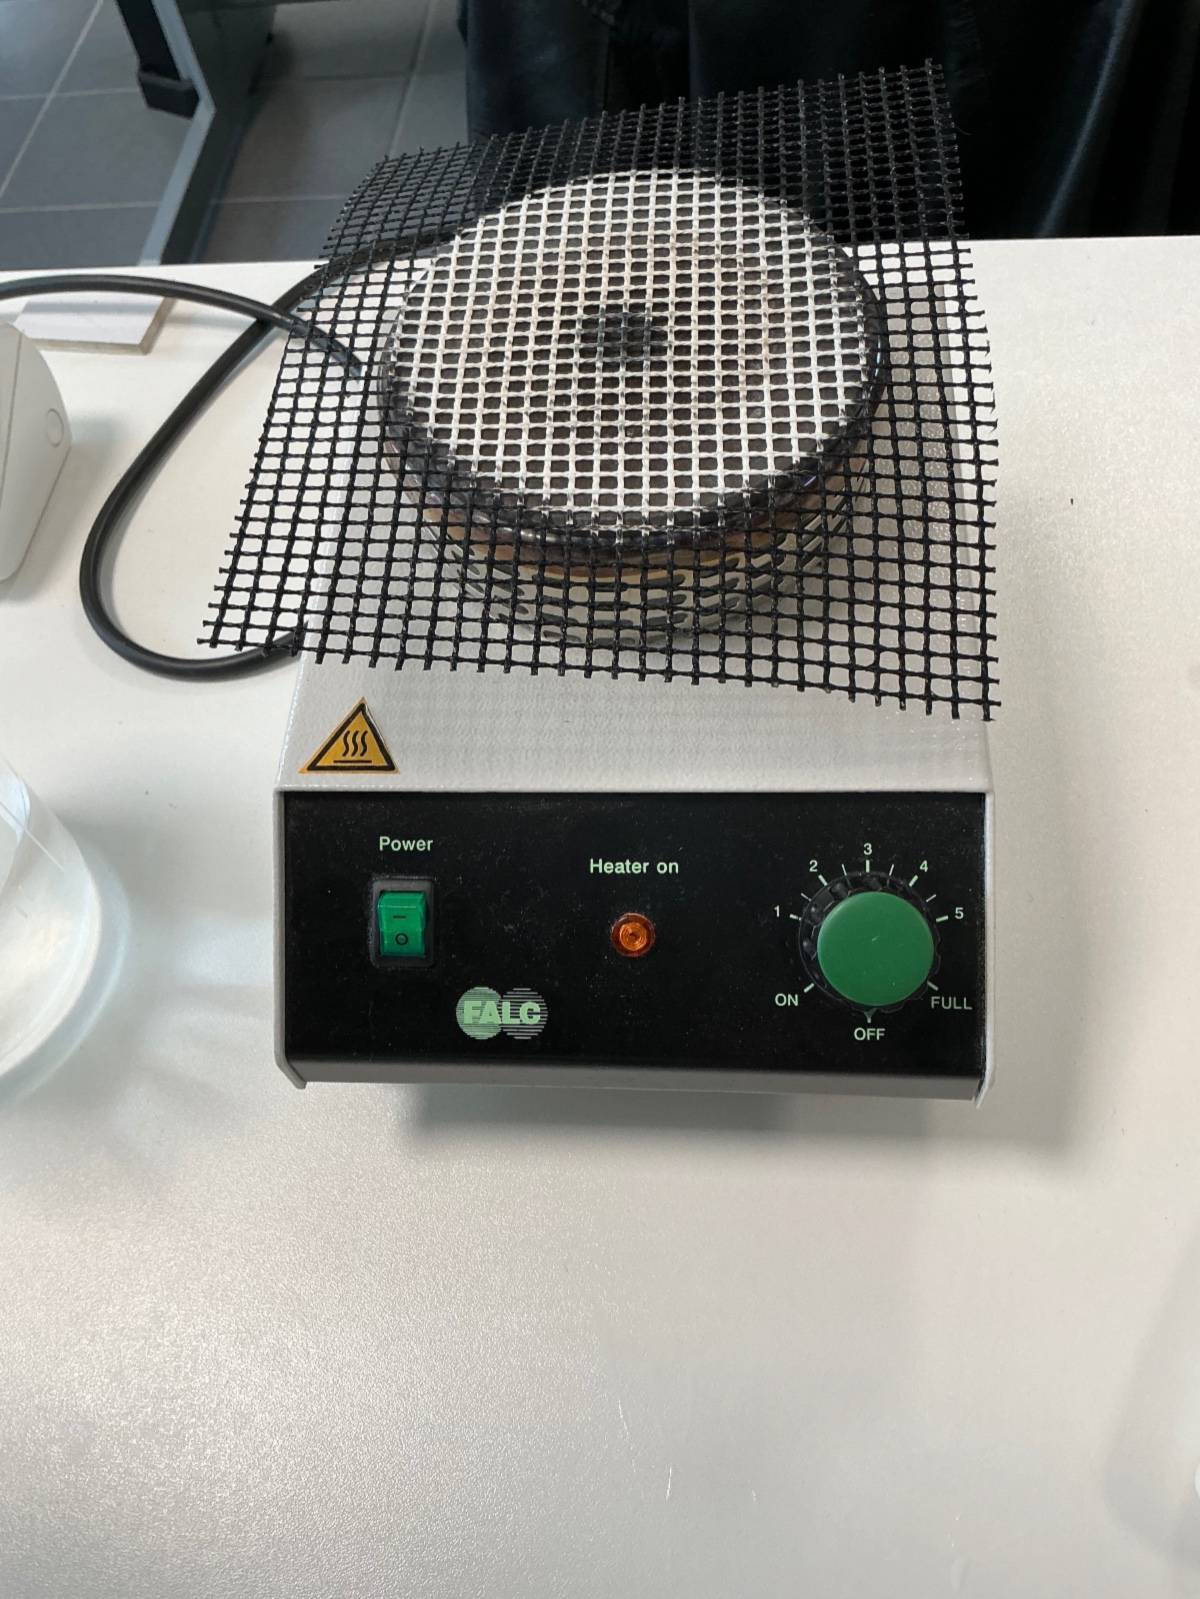
\includegraphics[width=0.30\textwidth]{6.jpg}
	\caption{Fornellino elettrico.}
\end{figure}

\begin{figure}[H]
	\centering
	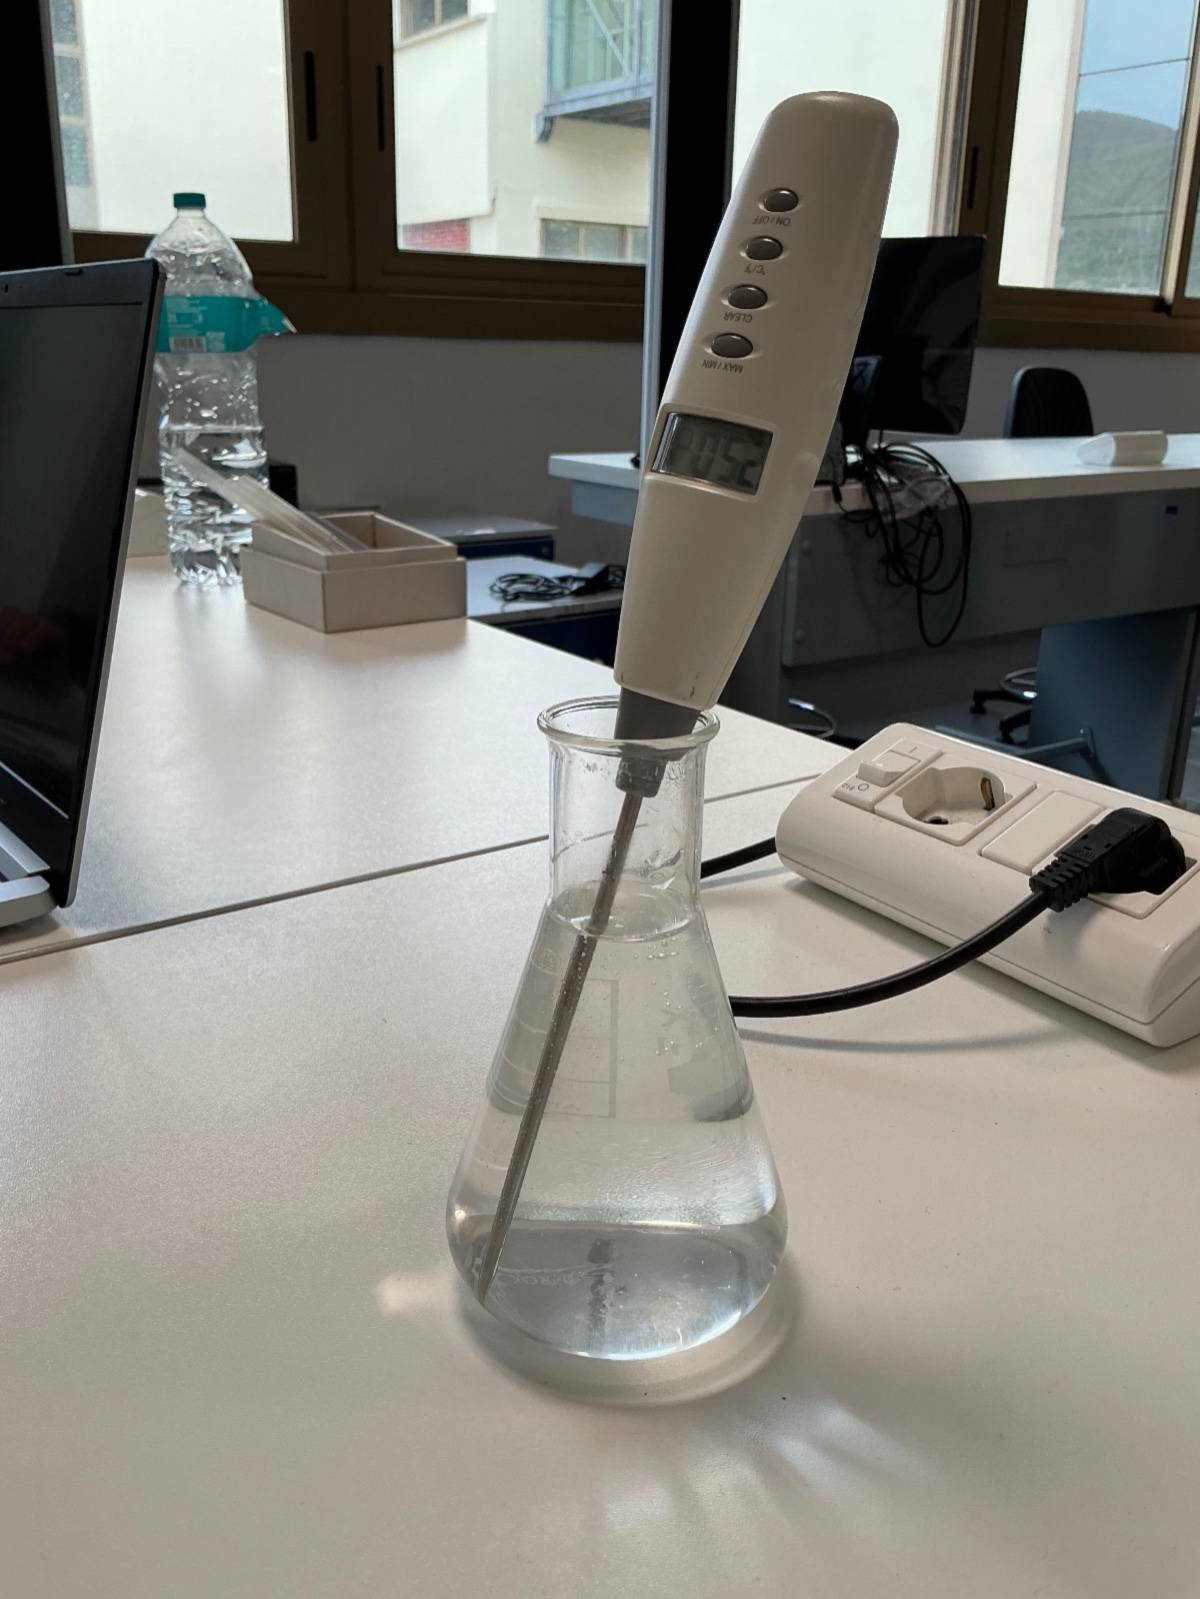
\includegraphics[width=0.30\textwidth]{2.jpg}
	\caption{Termometro digitale.}
\end{figure}

\begin{figure}[H]
	\centering
	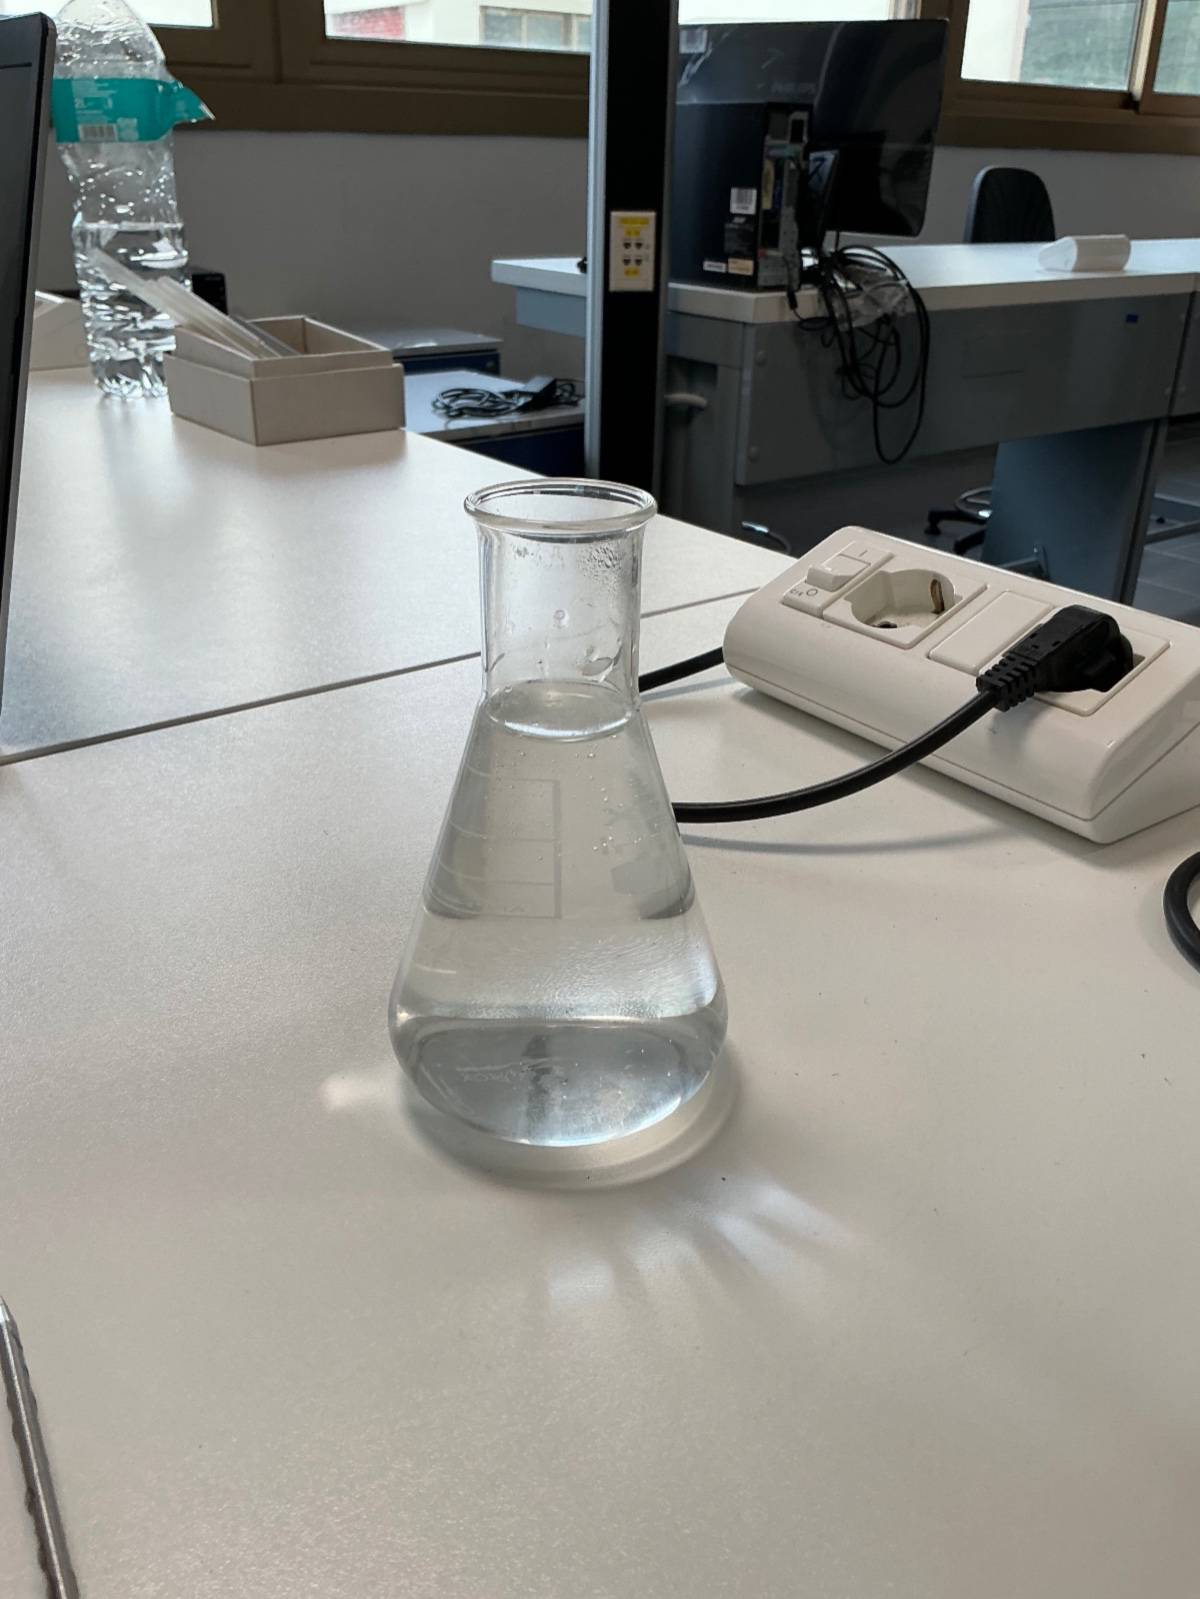
\includegraphics[width=0.30\textwidth]{4.jpg}
	\caption{Becher.}
\end{figure}

\begin{figure}[H]
	\centering
	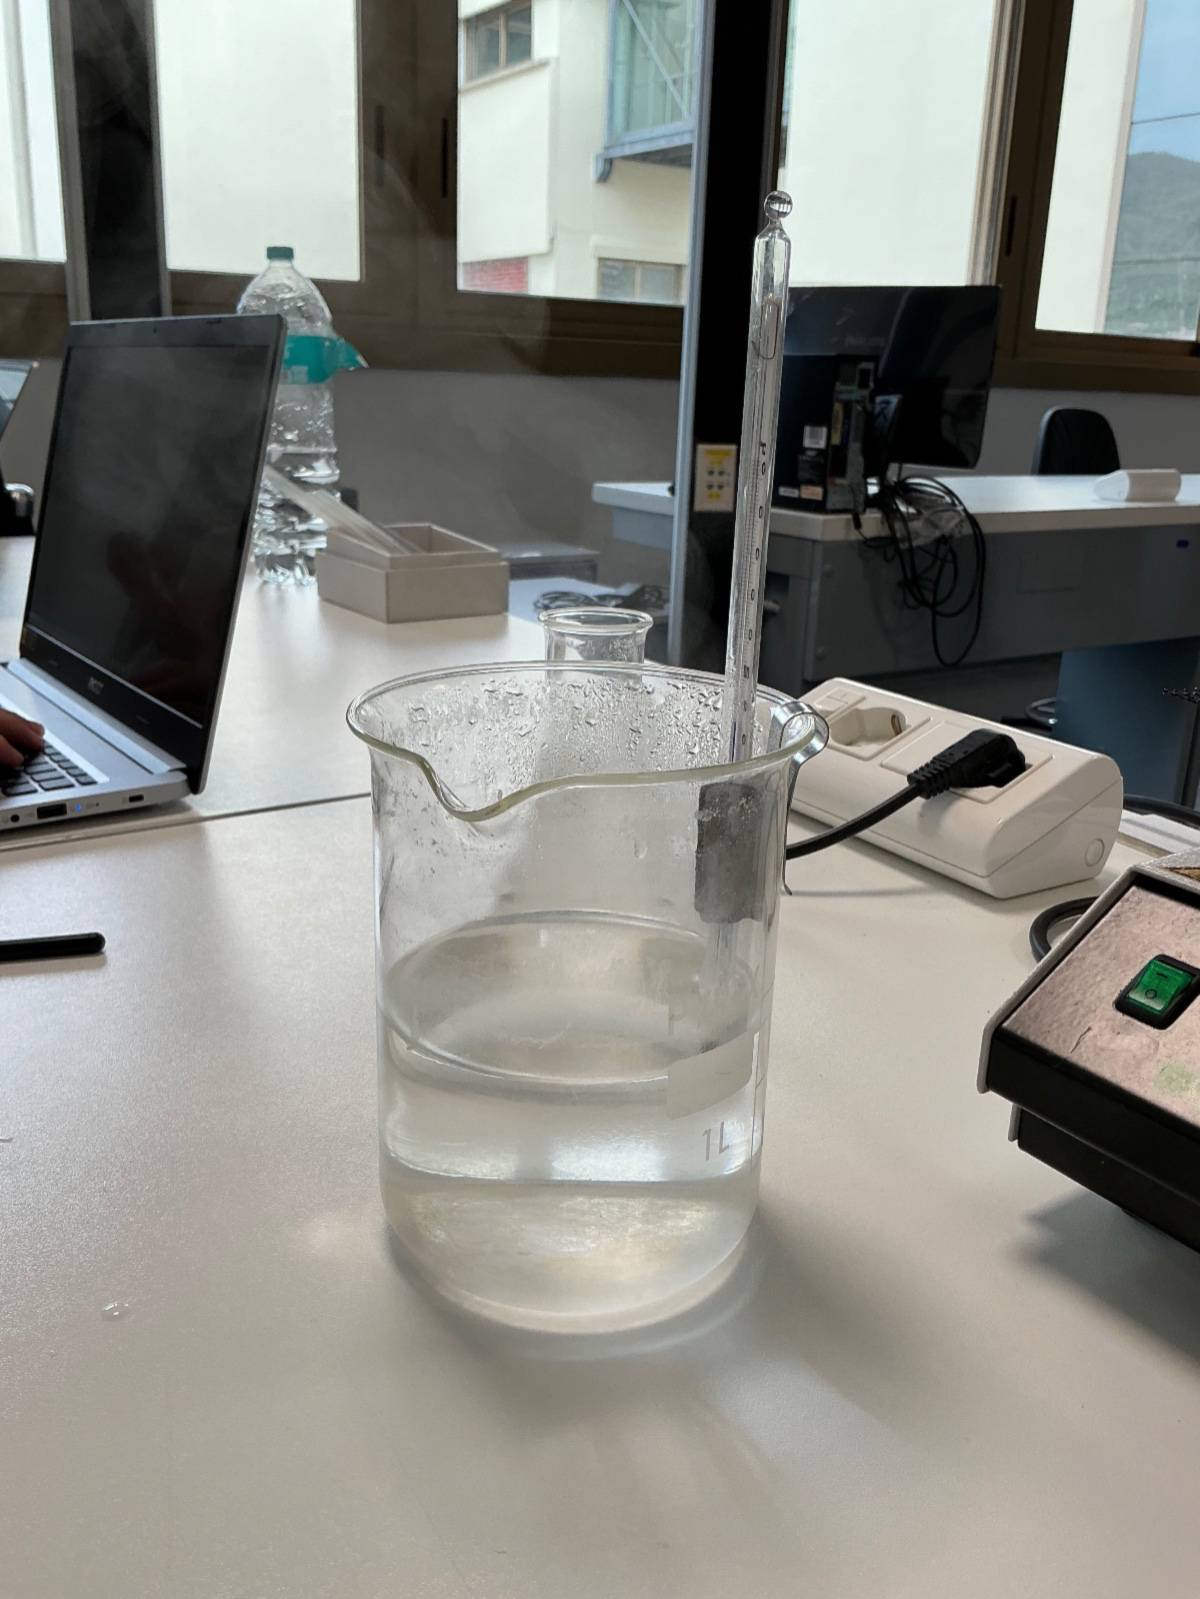
\includegraphics[width=0.30\textwidth]{5.jpg}
	\caption{Becher.}
\end{figure}